\documentclass[a4paper,sffamily,12pt]{article}

\usepackage[T1]{fontenc}
\usepackage[french]{babel}
\usepackage[utf8]{inputenc}

% Insertion d'image
\usepackage{graphicx}

% Création de lien
\usepackage[colorlinks,linkcolor=blue]{hyperref}

% Formatage des titres de sections
\usepackage{titlesec}
\titleformat{\section}
  {\normalfont\Large\bfseries\sffamily}{\thesection.}{0.33em}{}[\hrule]
\titleformat{\paragraph}
  {\normalfont\bfseries\sffamily}{\theparagraph.}{0.33em}{}
 
 % En-tête
\usepackage{fancyhdr}
\pagestyle{fancy}
\renewcommand\headrulewidth{1pt}
\fancyhead[L]{Web des données, web sémantique}
\fancyhead[R]{$X1I1030$}

% Permet de mettre du texte au dessus du titre
\usepackage{titling}
\renewcommand{\maketitlehooka}{\noindent COUILLEROT Carol \hfill \\ MAHIER Loïc \hfill \\ PHALAVANDISHVILI  Demetre}

% Titre
\title{\vspace{\fill}\LARGE\bfseries\sffamily Rapport de projet\protect\footnote{rapport réalisé sous \LaTeX} \vspace{\fill}}

\begin{document}

	\date{} % Supprime la date
	\maketitle % Affiche le titre

	\thispagestyle{fancy} % Permet de mettre le titre sur la page ''fancy''
	
	\newpage
			
	\renewcommand{\contentsname}{Sommaire}
	\tableofcontents
	
	\newpage
	
	\section{Introduction}

		\vspace{0.5cm}

		L’objectif de ce projet est de transformer des données ouvertes de l'Enseignement supérieur, de la Recherche et de l'Innovation (\url{https://data.esr.gouv.fr/FR/}) en données sémantiques et de lier ses données sémantisées aux données sémantisées de nos collègues. Pour ce faire nous avons choisi des données sur les budgets dédiés à la recherche et au transfert de technologie (R\&T) des collectivités territoriales. Ce rapport présente notre démarche, les problèmes que nous avons rencontré et la manière dont nous avons procédé pour les résoudres. Vous trouverez en annexe des captures d'écrans des divers éléments que nous présenterons dans ce rapport. Aussi voici le lien du github : \url{https://github.com/loic44650/WebSemantic_projet} sur lequel vous trouverez l'intégralité de notre travail. \\

		\vspace{0.5cm}
		
	\section{Présentation des données}				

		\vspace{0.5cm}
		
		En tout premier lieu décrivons nos données. Comme leur nom l'indique, ces données décrivent des budgets, en montant ou en pourcentage, attribués à la recherche et au transfert technologique. Ces budgets ont un objectif, un indicateur et un indicateur d'effort. L'objectif indique à quoi est destiné ce budget, les indicateurs, eux, renseignent sur son type. Ces budgets sont datés et ils proviennent de différentes collectivités françaises. Ces collectivités sont territoriales : ce sont des communes, des ECPI, des collectivités générales ou régionales. Et chacune d'entre elles est rattachées à une région française. A chaque région est associé un code région et on distingue les anciennes régions des nouvelles issues de la réforme des régions de 2015. Notons que certains budgets sont parfois à l’échelle de la France. 
				
		\vspace{0.5cm}
		
	\section{Sémantisation des données}				

		\vspace{0.5cm}
		
		\subsection{Nettoyage des données}
			
			\vspace{0.5cm}
			
			Les données étant choisies, il est désormais temps de les sémantiser. Cependant, un peu de ''nettoyage'' s'impose avant cela, en effet le jeu de données présente certains défauts à corriger. Ainsi nous avons dû normaliser les années, les budgets et les régions. Par exemple il y avait plusieurs régions que l'on trouvait avec différentes syntaxes, cela aurait posé des problèmes plus tard, notamment au niveau des requêtes. Autre défaut du jeu de données, la présence d'une valeur ''TOTAL FRANCE'' dans les régions qui prête à confusion. Nous avons donc créé en plus de la colonne région une colonne pays servant à distinguer les deux échelles géographiques. Enfin, nous avons créé une colonne pourcentage. En effet, il était auparavant spécifié entre parenthèse dans les champs ''indicateur'' et ''objectif'' si le budget en question est un montant (en euro) ou un pourcentage. Il est désormais possible de le savoir à l'aide d'un simple booléen dans la colonne pourcentage. Toutes ces modifications sont apportées dans le but de rentre le jeu de données davantage utilisable et ainsi de simplifier nos futures requêtes.
		
			\vspace{0.5cm}
		
		\subsection{Choix des ontologies}
		
			\vspace{0.5cm}
			
			Voila les modifications majeures apportées au jeu de données. Maintenant que les données sont ''propres'' et pleinement exploitables on peut les sémantiser. La première étape est d'identifier les ontologies adéquates. \\
		
			\indent On commence par distinguer que nous avons des données qui renseignent sur la région, la collectivité, l'année, le code, le pourcentage, etc. Pour ces données là, l'ontologie ''dbo'' propre à \url{http://wiki.dbpedia.org/} est intéressante : nous utilisons ainsi les prédicats ''dbo'' suivants : ''dbo:year'', ''dbo:country'', ''dbo:region'', ''dbo:code'', ''dbo:Organization'' et ''dbo:percentage''. Ces champs sont en effet assez simple pour certain : une année, un code et un pourcentage par exemple sont des prédicats basiques présents dans dbpedia qui nous satisfont et qui correspondent aux données sans perdre de l'information. De même, pour les régions qui sont référencées dans dbpedia. A contrario le prédicat ''dbo:Organization'' que nous utilisons pour les collectivités territoriales, générales et régionales n'est peut être pas le plus adéquat car assez vague. Mais nous l'avons conservé faute d'avoir trouvé mieux, toutefois nous aurions pu pour ce cas précis créer notre propre ontologie.  \\ 
		
			\indent Ensuite on remarque que le reste des données identifie un budget, sa valeur ou son pourcentage, son objectif et son application. Pour ce faire nous avons choisis d'utiliser l'ontologie ''frapo'' (\url{http://www.sparontologies.net/ontologies/frapo/source.html} qui sert précisemment à définir des budgets. En effet nous aurions pu par exemple encore utiliser des ontologies de dbpedia : cependant celles-ci ne permettaient pas d'avoir des prédicats assez précis pour définir le type de nos données.  Nous avons donc décidé d'utiliser ''frapo''. Ainsi nous avons besoin des prédicats suivants : ''frapo:BudgetInformation'', ''frapo:appliesFor'' et ''frapo:BudgetedAmount''.
		
			\vspace{0.5cm}
			
		\subsection{Écriture du ''construct''}
			
			\vspace{0.5cm}
		
			Passons à présent à l'écriture du fichier ''construct'' qui va générer nos données RDF à partir du fichier CSV. Celui-ci se fait assez facilement, nous allons le voir en détail en procédant par étape. On va y trouver trois morceaux, un premier avec tous les préfixes utilisés nommé ''PREFIX'', un deuxième nommé ''CONSTRUCT'' et un dernier nommé ''WHERE''. Une fois n'est pas coutume, commençons par le dernier. La clause ''WHERE'' va servir à récupérer les valeurs des différentes colonnes du jeu de données et à les attribuer à des variables à l'aide du mot clé ''BIND''. Variables que nous typons à la manière du XMLSchema. On définit ainsi par exemple le montant du budget comme un ''xsd:double'' et l'objectif comme un ''xsd:string''. Dans le même temps, on crée notre URI en ajoutant à une url que nous avons arbitrairement choisis autant de variable que nécessaire pour identifier chacun des tuples de notre jeu de données. L'objectif étant de ne pas avoir de doublon. Pour ce faire nous utilisons une conditionnelle (IF(BOUND(x,y))) puisque nous avons besoin d'un champ qui est parfois vide. Cela nous permet selon la situation de passer d'un modèle d'URI à un autre suivant la conditionnelle. \\
			
			\indent Passons à la clause ''CONSTRUCT''. Celle-ci est finalement triviale,  nous y appliquons simplement les prédicats définis un peu plus tôt à chacune des variables que nous avons créé dans la clause ''WHERE''.  Et il n'y a pas grand chose de plus à en dire. Terminons donc l'explication du fichier ''construct'' en présentant le premier morceau, à savoir celui qui énonce tous les préfixes. On y retrouve tous les liens vers les ontologies que l'on utilise : notamment vers dbo, frapo, rdf et xsd. \\
			
			\vspace{0.5cm}
			
		\subsection{Obtention des données au format RDF}
			
			\vspace{0.5cm}
	
			Maintenant notre fichier ''construct'' écrit, nous créons nos données RDF à l'aide de l'applet TARQL, via le terminal. Nous indiquons l'encodage de nos données, le caractère qui sert à délimiter les données, le fichier ''construct'', le fichier au format CSV contenant les données et enfin le fichier de destination des données RDF obtenu à l'aide d'un flux de redirection : \\
			
			\noindent tarql -e utf-8 --delimiter \textbackslash; construct.sparql data\_non\_semantiques.csv > data\_semantiques.rdf

			\vspace{0.5cm}

		\subsection{Écriture de quelques requêtes }
			
			\vspace{0.5cm}
	
			Les données étant sémantisés, il faut les tester. Pour ce faire nous avons choisi d'utiliser Apache-Jena Fuseki. C'est d'ailleurs l'outil que nous allons utiliser tout au long du projet pour tester nos diverses requêtes. Nous n'allons pas détailler ici toutes nos requêtes, cela n'aurait  pas d'intérêt. Nous en avons fait 5 sur notre jeu de données et nous avons essayé de varier leurs écritures en utilisant différentes syntaxes telles que des ''OPTIONAL'', des ''FILTER'', des ''SUM'', des ''ORDER BY'' et des ''GROUP BY''. Vous trouverez une description de chacune de ces requêtes dans le fichier ''queries.sparql'' de notre github.

			\vspace{0.5cm}
			
	\section{Liaisons des données}

		\vspace{0.5cm}
			
		\subsection{Présentation des jeux de données liés}
			
			\vspace{0.5cm}			

				Maintenant nos données propres, sémantisées et testées, il est temps de les lier à celles de nos camarades. Ainsi nous avons lié nos données à celles de deux autres groupes. Le premier groupe a des données qui portent sur les moyens consacrés à la R\&D par les entreprises. De ce fait, lier nos données à ce groupe nous permet d'avoir à l'échelle nationale à la fois les budgets publics (nous) et privés (eux). Des lors nous constatons qu'ils possèdent le code et le nom de chaque région, nous savons donc déjà sur quel attribut nous allons pouvoir lier nos données entre nous. C'est en gardant cet attribut en tête que nous avons cherché à lier nos données à un second groupe. Ce second groupe possède des données sur le nombre d'étudiants inscrits dans l'enseignement supérieur que nous avons évidemment lié à l'aide du code région. Ces données nous permettent de regarder si il y a un lien entre l'investissement dans la recherche et le nombre d'étudiants  par région (étudiant potentiellement destiné à être chercheur ). Nous constatons que beaucoup de groupes ont des données possédant le code région ou simplement le nom de la région. Il serait donc possible de lier énormément de jeux de données entre eux. Nous reviendrons dessus un peu plus tard et expliquerons pourquoi nous n'avons pas cherché à lier davantage de données entres elles. 

			\vspace{0.5cm}
			
		\subsection{Modification du ''construct''}
			
			\vspace{0.5cm}

			Expliquons à présent comment nous avons lié nos données entres elles. Nous l'avons fait pour deux jeux de données, mais la démarche étant identique, nous n'allons la présenter  qu'une fois. Précisons que celle-ci est vraiment identique, puisque nous faisons notre liaison à l'aide du code région pour les deux jeux de données. Ainsi si l'on procède de la même manière que pour la création du fichier ''construct'' de base, nous allons rajouter des éléments dans les clauses ''CONSTRUCT'' et ''WHERE''.  \\
			
			\indent Commençons encore par la clause ''WHERE'' : nous avons décidé de lier nos données via le code région, de fait il faut créer une URI concaténée à notre code région, URI qui devra être rajouté dans le fichier ''construct'' de l'autre groupe. De même il nous faut récupérer l'URI de l'autre groupe, ce dernier contient également le code région. Notez que c'est la variable ''codereg'' (issue du BIND) que nous ajoutons à l'URI. Nous avons dû pour ce point précis modifier notre ''BIND'' puisque le code région contenait au préalable un ''R'' suivit du code. Or, nos camarades ont uniquement le code région, sans ''R''. Nous avons donc utilisé la fonction ''STRAFTER'' pour récupérer dans notre variable ''codereg'' uniquement ce qui succède au ''R''. \\
			
			\indent Une fois cela fait, autrement dit une fois que l'on a spécifié les URIs que l'on va utiliser pour lier nos données, il faut dans la clause ''CONSTRUCT'', à présent, faire le lien entre les deux. Pour ce faire on y rajoute simplement une instruction spécifiant que le code région de notre URI est le même que celui de l'URI de l'autre groupe. Pour cela on utilise l'ontologie ''owl:sameAs''. Cela étant fait, nos données sont liés ou du moins pour nous. En effet ils devront eux aussi rajouter un URI pour récupérer notre code région  ainsi qu'utiliser ''owl:sameAs'' pour lier les URI. Après cela, les deux jeux de données seront liés dans les deux sens. \\
			
			\indent Comme indiqué au début nous n'allons pas détailler la démarche pour le second jeux de donnée. Cependant sachez qu'il faut encore récupérer son code région via son URI, et encore utiliser ''owl:sameAs'' pour lier nos données. De son coté l'autre groupe aura aussi besoin de notre code région, pour cela il peut réutiliser l'URI que nous avions créé pour la première liaison. \\
			
			\indent Voila désormais notre jeux de données lié à d'autres jeux de données. Essayons à présent d'en tirer quelque chose !
						
			\vspace{0.5cm}
			
		\subsection{Écriture d'une requête fédérée}
			
			\vspace{0.5cm}
			
			Notre requête a ainsi pour but d'afficher par région : le nombre d'étudiant dans l'enseignement supérieur, le budget public attribué à la recherche et le budget privé attribué à la recherche. Chacune des informations se trouvant dans un jeu de données différent. Nous devons donc faire une requête fédérée qui sera composée de deux clauses ''SERVICE''. En effet, on fait la somme des budgets publics sur notre jeu de données, puis on fait la somme des budgets privés sur le deuxième jeu de données et enfin on fait la somme des effectifs d'étudiants sur le dernier. Chacune de ces sommes se font par régions et par années. \\
			
			\indent Cette requête fédérée met plusieurs dizaines de minutes à s'exécuter avec seulement deux ''SERVICE'', c'est pourquoi nous n'avons pas cherché à lier davantage de jeux de données. Nous aurions été dans l'incapacité de les exploiter toutes en même temps et donc de produire des requêtes complexes et pertinantes sur l'ensemble.

			\vspace{0.5cm}			

	\section{Inférence}

		\vspace{0.5cm}
		
		Jusqu'ici nous avons définis grâce au langage RDF notre vocabulaire pour définir le budget d'une collectivité. En l'état il n'est pas possible de sortir des informations ne correspondant pas exactement à ce que l'on a demandé. Par exemple si l'on souhaite obetnir les budgets de recherche et transformation de la bretagne via la propriété ''dbo:Place'' le résultat est vide, car dans notre graphe RDF le lieu est rattaché au budget grâce à ''dbo:region''. Il faut donc créer une ontologie pour pouvoir raisonner sur nos données et pour ce faire nous avons utilisé le langage RDFS et le serveur apache Fuseki du framework Jena. Cela nécessite deux étapes : la définition du modèle puis la définition des règles.\\
		
		\indent Le modèle décrit les classes, les propriétés et les relations entre elles. Ainsi ''frapo:BudgetInformation'', ''dbo:Organization'' sont de type ''rdfs:Class'', mais ''dbo:percentage'' est de type ''rdf:Property''. \\ 
		
		\indent Les règles définissent les triplets de notre graphes à ajouter au résultat si certains triplets sont déjà présents dedans. En reprenant l'exemple précédent des budgets rattachés à la Bretagne, nous pouvons écrire la règle suivante : (?uri dbo:region ?region) -> (?uri dbo:place ?region) \\ 
		
		\indent Conséquemment les triplets '' ?uri dbo:region "Bretagne" '' seront insérés dans la liste des résultats. Cependant les données recueillies sur les budgets de recherche et de transformation ne se prêtent pas particulièrement à l'inférence car il y a peu d'interactions entre nos classes et propriétés.

		\newpage
				
	\section{Conclusion}

		\vspace{0.5cm}			

		\begin{figure}[!h]
			
			\centerline{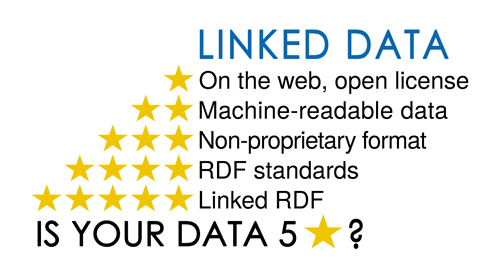
\includegraphics[height=6cm]{picture/linked_data.png}}
			\caption{5-stars program.sparql}
			\label{5stars}
			
		\end{figure}		
	
		\vspace{1cm}
		
		Pour conclure, parlons un peu du programme 5 étoiles. La première étoile impose que les données soit publiées sur le web sous licence ouverte. C'est le cas de nos données, puisque nous les avons obtenus sur le site open data du gouvernement français. La deuxième étoile impose que les données soit structurées, ce qui est le cas puisqu'elle sont sous format CSV. La troisième étoile impose que ces données soit sous un format non-propriétaire : CSV est un format non-propriétaire. La quatrième étoile impose d'utiliser des URIs et de suivre les standards RDF, c'est ce que nous avons fait. Et finalement vient la cinquième étoile, laquelle impose de lier les données. C'est également ce que l'on a fait. Ainsi, nous avons récupéré des données 3 étoiles et nous les avons rendu 5 étoiles.

		\newpage			
		
	\section{Annexe}

		\vspace{0.5cm}
		
		\begin{figure}[!h]
				
			\centerline{\includegraphics[height=17cm]{picture/constructv1.png}}
			\caption{Fichier Construct.sparql}
			\label{constructv1}
			
		\end{figure}		
	
		\newpage

		\begin{figure}[!h]
			
			\vspace{0.5cm}	
			\centerline{\includegraphics[height=17cm]{picture/constructv2.png}}
			\caption{Fichier Construct\_linked\_data.sparql}
			\label{constructv2}
			
		\end{figure}		
	
		\vspace{1cm}		
								
\end{document}
